\chapter{Solución propuesta}
\label{solucion}
\section{Arquitectura de la solución}
Hoy por hoy el desarrollo de Internet ha alcanzado niveles realmente impresionantes, no solo en lo respecta de los avances en capacidad de transición de datos y software que viven prácticamente en la red si no también su modelo de crecimiento y expansión en la sociedad post-moderna y de la era de de la información. Prácticamente no hay rincón del planeta en donde no pueda hoy en día llegar la la red de redes.\\
De acuerdo a las características del software y los requerimientos especificados, es de necesidad primaria implementar un sistema que pueda difundirse en la sociedad de manera masiva y velozmente, la RedSolLac quiere y debe poder llegar al mayor numero de personas interesadas en producir energías limpias y ojala pronto en el tiempo.\\
Planteados estos dos temas es que se ha tomado la decisión de realizar y desarrollar las soluciones basadas en plataformas web, se ha propuesto desarrollar un portal Web para la dilución de la Red el cual estar a cargo de un equipo externo al desarrollo de esta memoria pero el sistema desarrollado acá debe ser 100\% compatible con esta solución.\\
Dado que el portal Web de la RedSoLac estar implementado en el famoso CMS Wordpress he tomado la decisión de desarrollar las aplicación de forma modular en forma de plugins para este sistema Web.\\
Se desarrollaran 3 plugins cada uno debe satisfacer un requerimiento diferente de los cuales han sido planteados en el capitulo primero, estos plugins deberán cumplir estrictamente con el formato de desarrollo planteado en la documentación oficial de Wordpress.org y deberán funcionar como productos independientes y deberá poder ser portados a cualquier sistema con Wordpress.\\

\section{Wordpress}
Wordpress es una avanzada plataforma semántica de publicación personal orientada a la estética, los estándares Web y la usabilidad. Wordpress es libre y, al mismo tiempo, gratuito.\\
Wordpress es un sistema de manejador de contenidos (CMS del ingles Content Management Sistem) basado en estilo de publicaciones de blogs, además es un sistema libre de código abierto bajo la licencia GPL2. Esta echo en lenguaje PHP y utiliza el motor de bases de datos MySql, su arquitectura esta pensada y diseñada de forma modular, cosa que le permite adaptarse y ser configurable de acuerdo con los requerimientos de cada usuario.\\
La primera versión de esta plataforma fue liberada el año 2003 por Matt Mullenweg y es un rama del otro proyecto llamado b2/cafelog. Actualmente esta plataforma esta en su versión 3.0 y ha sido descargada mas de 65 millones de veces. se estima que Wordpress a la fecha es la herramienta de publicación de contenido mas utilizada y mas popular de la Red con aproximadamente un 14\% de participación en Internet y mas del 22\% de sitios nuevos o que se publican por primera vez.

\subsection{Arquitectura de Wordpress}
Tal como se menciono el apartado anterior Wordpress es una potente plataforma para la publicación de sitios en la Web. la plataforma esta programada en el lenguaje PHP y utiliza el motor de bases de datos MySql, para la parte visual utiliza hojas de estilo CSS.\\
Wordpress esta echo de tal manera que permita a sus usuario modificar o configurar partes esenciales del sistema que permitan gran funcionalidad y adaptación a los requerimientos del sistema, además cuanta con un framework y una API que permiten a programadores realizar aplicación de manera muy sencilla para que se adapten a la plataforma.

\subsection{Themes}
La parte visual o gráfica de esta plataforma funciona a través de un sistema llamado themes.\\

Los themes son un conjunto de librerías programadas en PHP que permiten estructura la forma en que se mostraran los contenidos del sitio y a la ves la gráfica que este expondrá a sus visitantes sin alterar el contenido del sitio. Wordpress al estar diseñado de manera modular permite a sus usuarios contar con gran cantidad de themes diferentes y mediante una interfaz de administración permite intercambiar estos themes de manera rápida y sencilla. Adicionalmente en el mercado existe extensos depósitos de themes que pueden ser instalados en cualquier sitio compatible con la versión indicada de Wordpress.\\

En el sitio de Wordpress podemos encontrar una extensa documentación y un API bien estructura que indica a los programadores que deseen desarrollar nuevos themes como deben estructurar el paquete de librerías y que funcionalidades pueden agregar o quitar. Adicionalmente estas librerías pueden posteriormente publicarse libremente o bien Wordpress da la libertad a sus usuarios de vender trabajos basados en su framework.

\subsection{Plugins}
Los plugins funcionan casi de la misma manera que los themes y así también la mayoría de los componente que dispone Wordpress. Estos son un conjunto de librerías programadas en PHP que pueden instalarse o desinstalares desde el panel de administración.\\

Cada plugins esta diseñado para agregar nuevas funcionalidades al los sitios, la documentación de Wordpress entrega pautas estrictas de como deben estar programadas las libreáis para que las nuevas funcionalidades no interfieran con el funcionamiento normal del sistema. Un plugins además puede modificar casi cualquier funcionalidad del sistema siempre que no interfiera con funciones criticas.

\subsection{Widgets}
Los widgets son pequeños programas autónomos que permiten agregar nuevas funcionalidades al sistema pero que adicional a un plugins común y corrientes posee de una interfaz visual y esta diseñado para exponer al usuario algún dato o funcionalidad especifica. Estos pequeños programas pueden agregarse y quitarse manera muy rápida y pueden y tienen la característica de ser móviles. Generalmente son programas que se agregan en las barras laterales.

\subsection{Multiusuario}
Wordpress permite la creación y administración de mucho usuarios los cuales pueden tener diferentes responsabilidades dentro del sistema tales como administrar el contenido o bien administrar la conflagración del sitio. esto permite que la mantención del sitio y a la vez las responsabilidades pueda estar muy bien distribuidas sin riesgo de que algún usuario realize tareas no permitidas por si nivel de acceso.

\section{PHP}
PHP es un acrónimo recursivo que significa PHP Hypertext Pre-processor. Fue creado originalmente por Rasmus Lerdorf en 1994; sin embargo la implementación principal de PHP es producida ahora por The PHP Group y sirve como el estándar de facto para PHP al no haber una especificación formal. Publicado bajo la PHP License, la Free Software Foundation considera esta licencia como software libre.\\

Es un lenguaje de programación interpretado (Lenguaje de alto rendimiento), diseñado originalmente para la creación de páginas web dinámicas. Se usa principalmente para la interpretación del lado del servidor (server-side scripting) pero actualmente puede ser utilizado desde una interfaz de línea de comandos o en la creación de otros tipos de programas incluyendo aplicaciones con interfaz gráfica.

\begin{itemize}
\item Orientado al desarrollo de aplicaciones web dinámicas con acceso a información almacenada en una base de datos.
\item El código fuente escrito en PHP es invisible al navegador web y al cliente ya que es el servidor el que se encarga de ejecutar el código y enviar su resultado HTML al navegador. Esto hace que la programación en PHP sea segura y confiable.
\item Capacidad de conexión con la mayoría de los motores de base de datos que se utilizan en la actualidad, destaca su conectividad con MySQL y PostgreSQL.
\item Capacidad de expandir su potencial utilizando módulos.
\item Posee una amplia documentación en su sitio web oficial, entre la cual se destaca que todas las funciones del sistema están explicadas y ejemplificadas en un único archivo de ayuda.
\item Es libre, por lo que se presenta como una alternativa de fácil acceso para todos.
\item Permite aplicar técnicas de programación orientada a objetos.
\item Biblioteca nativa de funciones sumamente amplia e incluida.
\item No requiere definición de tipos de variables aunque sus variables se pueden evaluar también por el tipo que estén manejando en tiempo de ejecución.
\item Tiene manejo de excepciones (desde PHP5).
\item Si bien PHP no obliga a quien lo usa a seguir una determinada metodología a la hora de programar (muchos otros lenguajes tampoco lo hacen), aun haciéndolo, el programador puede aplicar en su trabajo cualquier técnica de programación o de desarrollo que le permita escribir código ordenado, estructurado y manejable. Un ejemplo de esto son los desarrollos que en PHP se han hecho del patrón de diseño Modelo Vista Controlador (MVC), que permiten separar el tratamiento y acceso a los datos, la lógica de control y la interfaz de usuario en tres componentes independientes.
\end{itemize}

\section{MySql}
MySQL es un sistema de gestión de bases de datos relacional, multihilo y multiusuario con más de seis millones de instalaciones. MySQL AB ,desde enero de 2008 una subsidiaria de Sun Microsystems y ésta a su vez de Oracle Corporation desde abril de 2009, desarrolla MySQL como software libre en un esquema de licenciamiento dual.
Por un lado se ofrece bajo la GNU GPL para cualquier uso compatible con esta licencia, pero para aquellas empresas que quieran incorporarlo en productos privativos deben comprar a la empresa una licencia específica que les permita este uso. Está desarrollado en su mayor parte en ANSI C.\\

Al contrario de proyectos como Apache, donde el software es desarrollado por una comunidad pública y los derechos de autor del código están en poder del autor individual, MySQL es patrocinado por una empresa privada, que posee el copyright de la mayor parte del código.\\
Esto es lo que posibilita el esquema de licenciamiento anteriormente mencionado. Además de la venta de licencias privativas, la compañía ofrece soporte y servicios. Para sus operaciones contratan trabajadores alrededor del mundo que colaboran vía Internet. MySQL AB fue fundado por David Axmark, Allan Larsson y Michael Widenius.

\begin{itemize}
\item Usa GNU Automake, Autoconf, y Libtool para portabilidad
Uso de multihilos mediante hilos del kernel.
\item Usa tablas en disco b-tree para búsquedas rápidas con compresión de índice.
\item Tablas hash en memoria temporales.
\item El código MySQL se prueba con Purify (un detector de memoria perdida comercial) así como con Valgrind, una herramienta GPL.
\item Completo soporte para operadores y funciones en cláusulas select y where.
\item Completo soporte para cláusulas group by y order by, soporte de funciones de agrupación
\item Seguridad: ofrece un sistema de contraseñas y privilegios seguro mediante verificación basada en el host y el tráfico de contraseñas está cifrado al conectarse a un servidor.
\item Soporta gran cantidad de datos. MySQL Server tiene bases de datos de hasta 50 millones de registros.
\item Se permiten hasta 64 índices por tabla (32 antes de MySQL 4.1.2). Cada índice puede consistir desde 1 hasta 16 columnas o partes de columnas. El máximo ancho de límite son 1000 bytes (500 antes de MySQL 4.1.2).
\item Los clientes se conectan al servidor MySQL usando sockets TCP/IP en cualquier plataforma. En sistemas Windows se pueden conectar usando named pipes y en sistemas Unix usando ficheros socket Unix.
\item En MySQL 5.0, los clientes y servidores Windows se pueden conectar usando memoria compartida.
\item MySQL contiene su propio paquete de pruebas de rendimiento proporcionado con el código fuente de la distribución de MySQL.
\end{itemize}

\section{CSS}
El nombre hojas de estilo en cascada viene del inglés Cascading Style Sheets, del que toma sus siglas. CSS es un lenguaje usado para definir la presentación de un documento estructurado escrito en HTML o XML. El W3C (World Wide Web Consortium) es el encargado de formular la especificación de las hojas de estilo que servirán de estándar para los agentes de usuario o navegadores.\\

La idea que se encuentra detrás del desarrollo de CSS es separar la estructura de un documento de su presentación.
La información de estilo puede ser adjuntada como un documento separado o en el mismo documento HTML. En este último caso podrían definirse estilos generales en la cabecera del documento o en cada etiqueta particular mediante el atributo "<style>".

\section{Hardware}
Durante el desarrollo e implementación del software involucrado en esta memoria fue necesario aprender e interiorizarse con una serie de elementos de hardware que forman parte de la mayoría de las estaciones de monitoreo para plantas de energía solar así como elementos comunes empleados en la construcción de estas mismas.\\

La principal estación de monitoreo utilizada para la realización de las pruebas de software se ubica en el techo del edificio principal de fundación chile en la región metropolitana comuna de Vitacura, esta estación cuenta con los siguientes componentes:

\subsection{Datalogger Campbell CR1000}
\begin{figure}[h!]
	\centering
	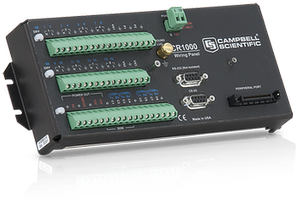
\includegraphics[width=100pt]{images/cr1000}
	\caption{Datalogger Campbell CR1000}
\end{figure}
 
Un Datalogger es un pequeño computador que cuenta con diferentes entradas para la conexión de sensores y otros equipos electrónicos, además cuenta con un sistema operativo que mediante el software correcto permite ingresar scripts para controlar su funcionamiento, además de sensores es posible conectar una serie de periféricos que cumplen diferentes funciones tales como módems, teclados o pantallas.\\

Datalogger CR1000 es compacto y ligero tiene una velocidad de ejecución de programa de 100 Hz y 1500 Hz en burstmode. En su interior, un procesador de 16-bit H8S Hitachi con 32-bit en la arquitectura interna de la CPU.
Ocho entradas analógicas diferenciales (16 single-ended), dos canales contadores
de pulsos y ocho puertos digitales I/O ports complementados con los puertos CS I/O y RS-232, puerto de 40-pin para periféricos y opción Ethernet.

Campbell scientific es una compañía dedicada a la construcción y distribución de estos equipos. Junto con los equipos mantiene y provee un lenguaje de programación llamado CRBasic el cual esta basado en Basic, mediante este lenguaje es posible crea diferentes scripts de control que permiten manejar el comportamiento del Datalogger, como es por ejemplo los datos necesarios a capturar proveniente de los diferentes sensores y el envió de datos a través de un módem gprs u interfaz Ethernet. 

\begin{itemize}
\item Ideal para aplicaciones en medición solar, vientos, estaciones meteorológicas, calidad del aire, humedad del suelo, nivel de agua, prevenciones de avalanchas y otros.
\item Comunicación serial, dispone de entradas para dispositivos E/S.
\item Recolecta y almacena datos además puede controlar periféricos y actuar como sistema central.
\item Flexibilidad de alimentación energética y sistemas de comunicación, lo que lo hace ideal para instalaciones remotas.
\item 4 MB de memoria interna y puede ser expandido con módulos adicionales.
\item Soporta protocolos PakBus, Modbus, SDI-12, y DNP3.
\item Dispone de canales de expansión para periféricos lo que hace posible agregar funcionalidades al sistema.
\item Compatible con software LoggerNet, PC400, o ShortCut.
\item Protocolos de comunicación: TCP/IP, email, FTP, servidor web.
\item Entradas protegidas mediante tubos de descarga de gas(Gas Discharge Tube (GDT)).
\end{itemize}

\subsection{Interfaz Ethernet NL200 Campbell}

\begin{figure}[h!]
        \centering
        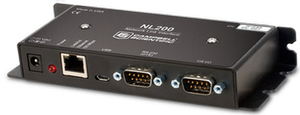
\includegraphics[width=100pt]{images/nl200}
        \caption{Periférico Campbell NL200} 
\end{figure}

Esta interfaz es un periférico distribuido por Campbell scientific al igual que el Datalogger mencionado anteriormente, este periférico permite anexar una interfaz Ethernet directamente al Datalogger de manera de permitir la conexión a la red Ethernet de manera directa. Es mediante este aparato que la información recopilada de la Estación de monitoreo Fch Vitacura envía los datos al servidor donde se alojan las aplicaciones desarrolladas y la base de datos.\\

Como característica adicional hay que mencionar que es un periférico diseñado especialmente para funcionar con el Datalogger antes mencionado y además es un periférico pensado para un consumo de energía muy bajo, lo que lo hace ideal para estar conectado a la batería de la estación.

\begin{itemize}
\item Conector de corriente: DC Barrel
\item Requerimientos de corriente: 7 to 20 Vdc 
\item Consumo de corriente: 50 mA active @ 13 Vdc;
\item Standby forzado al tener 2 mA de corriente cuando esta conectado al puerto CS I/O en modo Bridge.
\item Rango de temperatura en operación : ${-25}^{\circ}$ to ${+50}^{\circ}C$
\item Configuración: Puede ser configurado a través de USB o Ethernet, mediante Telnet.
\item Puerto CS I/O: SDC 7, 8, 10, or 11
\item Puerto RS-232: DTE
\item Puerto USB: Micro-B
\item Puerto Ethernet: IEEE 802.3, Auto-MDIX, IPv4, TCP, DHCP, Ping, Telnet, TLS, PakBus
\item Dimensiones: 16 x 6.73 x 2.54 cm.
\item Peso: 177 g
\item Puerto RS-232 DTE: 1200 hasta 115.2k bps
\item Puerto CS I/O: 9600 hasta 460.8k bps
\item Ethernet: 10/100 Mbps
\end{itemize}

\subsection{MultiModem GPRS Multitech modelo MTCBA-G-F4}

\begin{figure}[h!]
        \centering
        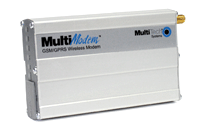
\includegraphics[width=100pt]{images/MultiModemGPRS}
        \caption{MultiModem Multitech MTCBA-G-F4} 
\end{figure}

Este periférico construido y distribuido por Multitech es un módem que permite conectarse a una red GSM y obtener conexión GPRS, este módem funciona en conjunto con el Datalogger Campbell de la misma forma que lo hace el periférico NL200 salvo que este aparato provee al Datalogger de una conexión a la Red de manera inalámbrica permitiendo conectar estaciones de monitores e lugares remotos del país.\\
Para poder operar con este módem es necesario tener contratado un plan de datos de telefonía móvil con alguna de las compañías que operan en el sector donde se instalan las estaciones de monitoreo.

\begin{itemize}
\item GPRS Clase 10.
\item Banda cuádruple GSM 850/900/1800/1900 MHz.
\item Corrección de errores MNP 2, Compresión V.42bis.
\item Packet data up to 85.6K bps.
\item Pila TCP/IP embedida.
\item Conector de antena SMA.
\item 2 años de garantía.
\end{itemize}

\subsection{Piranómetro PSP-Eppley}

\begin{figure}[h!]
        \centering
        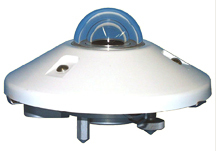
\includegraphics[width=100pt]{images/piranometro}
        \caption{Piranómetro psp-eplay} 
\end{figure}

El Piranómetro de Precisión Espectral es un instrumento de medición de clase mundial designado para medir la radiación entregada por el sol y l atmósfera, para todo el espectro eléctrico o bien puede configurarse para un segmento especifico.\\
Se compone de una multi unión circular de hilo bobinado junto a una termopila Eppley que tiene la capacidad de soportar fuertes vibraciones y choques mecánicos.

\subsection{Sensor de temperatura y humedad HMP60}
Es una sonda de humedad sencilla, económica y duradera. Es adecuada para aplicaciones de volumen, integración en equipos de otros fabricantes, incubadoras, cajas de manipulación con guantes, invernaderos, cámaras de fermentación y registradoras de datos.

\subsection{Batería PS100}

\begin{figure}[h!]
        \centering
        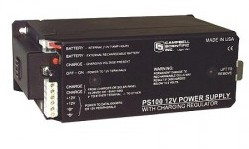
\includegraphics[width=100pt]{images/bateria}
        \caption{Batería PS100} 
\end{figure}

Baterías de plomo-ácido, la fuente de alimentación cuenta con un regulador de carga, puertos libres con salidas DC 12V, además de un conector para el módulo fotovoltaico.

\subsection{Panel fotovoltaico SX310M}

\begin{figure}[h!]
        \centering
        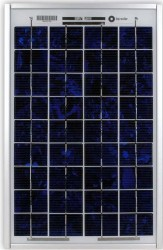
\includegraphics[width=100pt]{images/panelSolar}
        \caption{Panel Solar SX310M} 
\end{figure}

Modulo fotovoltaico de alta eficiencia, compuesto por celdas de nitrito de silicio multicristalinas.
\begin{itemize}
\item Tensión: 12.00 V
\item Potencia: 10 W
\item Corriente de salida: 0.59 mA
\item Largo: 10.59 pulgadas
\item Alto: 16.57 pulgadas
\item Grosor: 0.9 pulgadas
\item Peso: 1.49 Kg 
\end{itemize}

\subsection{Estación de monitoreo Solar Fch Vitacura}
\subsection{Estación de monitoreo Solar Norte}

\section{Diseño de la solución}
\subsection{Plugin gráficos solares}
\subsection{Plugin calculadora solar}
\subsection{Widget solar}

\section{Descripción detallada del sistema}


